\chapter{Trabalho Desenvolvido} \label{chap-desenvolvimentoWS}

O trabalho desenvolvido visa permitir que a plataforma Jason possa
ter tanto ambiente quanto agentes implementados em outras linguagens. Assim, a
plataforma Jason pode ser considerada uma arquitetura totalmente aberta, dado
que, até o raciocínio dos agentes poderia ser feito fora da plataforma.
A explicação de qual dos protocolos foi escolhido debatendo os critérios
utilizados e a estrutura de métodos necessários no servidor será explicado na
seção \ref{sec-WSS}. O cliente desses métodos fica localizado dentro da
plataforma Jason e os detalhes da implementação podem ser vistos na seção
\ref{sec-WSC}.

\section{Servidor de Serviços Web} \label{sec-WSS}

No capítulo \ref{chap-introducao} foi comentado que tanto SOAP quanto XML-RPC são
mecanismos comuns para o conjunto de linguagens escolhidos, pois não importa
qual deles se escolha haverá sempre pelo menos uma biblioteca para uso. Assim,
o critério decisivo utilizado para decidir foi a simplicidade, visto que
isso reflete nas mensagens e na curva de aprendizagem. Por exemplo,
desconsiderando os dados entregues nas mensagens trocadas tem-se que o SOAP
envia 472 bytes e o XML-RPC 173 bytes. Além disso, a curva de aprendizagem
do XML-RPC é menor pois há quase seis vezes menos tipos de dados que o
padrão SOAP.

\begin{figure}[h]
               \begin{center}
               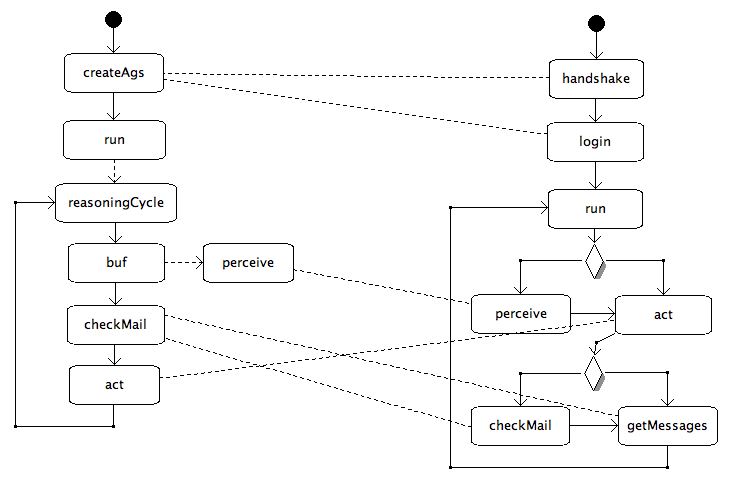
\includegraphics[width=104mm]{figuras/implXR-ag-compare-cycle.png}
                \end{center}
                \caption{Diagrama relacionando o ciclo do agente Jason (esquerda) com os métodos à serem implementados em serviços (direita).}
                \label{fig-uml-ag-cycle}
\end{figure}

Com o protocolo a ser utilizado definido, tudo que resta é definir como os
agentes e o ambiente podem ser implementados utilizando WS. Um servidor sempre
representa uma coleção de entidades do seu tipo determinado. No caso do
ambiente deve-se lembrar que todos os métodos influenciarão um único ambiente
compartilhado por diversos agentes.

\begin{table}
	\caption{Definição dos métodos obrigatórios no servidor de agentes.}
	\label{table-server-agents}
	\begin{center}
	\begin{tabular}{|p{34mm}|p{50mm}|p{50mm}|} % 140mm
		\hline
		Método & Parâmetros & Descrição \\ \hline
		handshake & Desafio (String). & Resolve um desafio proposto. \\ \hline
		login & Nome do agente (String). & Devolve um identificador (ID) numérico do agente. \\ \hline
		logout & ID (Numero) & Libera o ID associado com um determinado agente. \\ \hline
		perceive & ID (Numero) e Percepções (Array) & Associa um conjunto de percepções e retorna a ação do agente especificado.\\ \hline
		act & ID (Numero) e Esvaziar percepções (Boolean) & Esvazia as percepções do agente e retorna sua ação. \\ \hline
		checkMail & ID (Numero) e Mensagens (Array) & Entrega as mensagens
novas e retorna as mensagens à serem enviadas aos outros agentes.\\ \hline
		getMessages & ID (Numero) & Retorna todas as mensagens à serem enviadas aos outros. \\ \hline
	\end{tabular}
	\end{center}
\end{table}

Na Tabela~\ref{table-server-agents} há as definições sobre os métodos
obrigatórios a serem implementados no lado do servidor. Esses métodos são
chamados pela plataforma Jason em momentos específicos para operar o agente.
Os métodos \emph{handshake} e \emph{login} são chamados durante a criação do
agente na inicialização da plataforma Jason. O primeiro método recebe um
desafio (uma string qualquer) e deve responder o desafio da forma esperada.
Desse modo, a plataforma Jason sabe que o WSS sendo utilizado tem o mínimo de
confiabilidade exigido. O segundo método, \emph{login}, serve para associar um
identificador único com determinado agente. Esse identificador é utilizado nas
chamadas seguintes da plataforma Jason. Ao término da plataforma Jason a
função \emph{logout} é chamada para liberar o identificador único
criado.%\dev{hoje nao ha protecao aqui e nao tera}

Todo agente se comunica com outros agentes em algum nível, seja ela de forma
direta (recebendo uma mensagem de outro) ou indireta (alterações de percepções
do ambiente). Para a comunicação direta existir entre agentes fora da
plataforma Jason, existem os métodos \emph{checkMail} e \emph{getMessages}. O
método \emph{checkMail} entrega as mensagens novas para o agente e, ao fim,
chama \emph{getMessages} para devolver todas as mensagens que o agente deseja
enviar para os demais agentes. Note que, se o agente não tiver novas mensagens
à serem recebidas, a plataforma pode chamar de maneira direta a função para
consultar as mensagens à serem enviadas. Esse comportamento é observado na
Figura~\ref{fig-uml-ag-cycle}.

Quanto a forma de comunicação indireta, os agentes percebem modificações no
mundo através de ``sensores'' que refletem as percepções que o agente tem
sobre as coisas no ambiente. De forma análoga às mensagens, as percepções são
alteradas pelo método \emph{perceive}. Esse método serve para cadastrar o
estado atual conhecido do ambiente e tem como retorno uma ação que deve ser
executada no ambiente através do método \emph{act}. A plataforma Jason decide
chamar \emph{act} ao invês de \emph{perceive} quando não houver alterações nos
sensores do agente ou quando não há percepção de nenhum dos sensores (conjunto
vazio).

Na Tabela~\ref{table-server-environment} tem-se a descrição dos métodos
mandatórios para implementação de um WSS como ambiente. Esses métodos lidam em
grande parte com percepções que serão explicados mais adiante. Quando, na
inicialização da plataforma, o agente precisa de informações dos seus
``sensores'' é feita a chamada para o método \emph{handshake}. Ele trabalha da
mesma maneira que o WSS do agente. As funções que adicionam
(\emph{addPercept}), removem (\emph{removePercept}) ou
esvaziam (\emph{clearPercepts}) o conjunto de percepções são aos pares para
deixar claro quando opera no conjunto comum ou específico (são as mesmas
funções, mas terminadas com a palavra Local).

\begin{table}
	\caption{Definição dos métodos obrigatórios no servidor do ambiente.}
	\label{table-server-environment}
	\begin{center}
	\begin{tabular}{|p{34mm}|p{50mm}|p{50mm}|} % 140mm
		\hline
		Método & Parâmetros & Descrição \\ \hline
		handshake & Desafio (String). & Resolve um desafio proposto. \\ \hline
		addPercept & Percepção & Insere uma percepção para todos os agentes.\\ \hline
		addPerceptLocal & Nome do agente (String) e Percepção. & Insere uma percepção para um agente específico. \\ \hline
		clearPercepts & Sem parâmetros. & Apaga as percepções comuns à todos os agentes.\\ \hline
		clearPerceptsLocal & Nome do agente (String). & Apaga as percepções específicas de um agente.\\ \hline
		havePercepts & Nome do agente (String). & Há ou não percepções novas. \\ \hline
		getPercepts &  Nome do agente (String) e envio atualizado (Boolean). & Retorna todas as percepções do agente. \\ \hline
		removePercept & Percepção. & Retira uma percepção comum de todos os agentes. \\ \hline
		removePerceptLocal & Nome do agente (String) e Percepção. & Retira uma percepção que é específica de um agente. \\ \hline
		performAction & Nome do agente (String) e Ação. & O agente executa a ação especificada. \\ \hline
	\end{tabular}
	\end{center}
\end{table}

A recuperação das percepções é feita unicamente via chamada ao método
\emph{getPercepts}. Esse método, quando chamado, recebe o agente operando para
conseguir montar o conjunto de percepções do mesmo e se deve considerar
isso como a percepção do ciclo do Jason para computar como atualização. O
conjunto de percepções enviado é o conjunto comum ou global de percepções
unido com o conjunto de percepções locais ou específicas do agente informado.
O método \emph{havePercepts} serve para informar a plataforma que há novas
percepções ou não, assim a mesma sabe quando pegar as percepções.

Durante toda a simulação o agente realiza alguma ação, seja no ambiente ou
não. Essas ações são realizadas utilizando o método \emph{performAction} que
recebe o agente (executor) e a ação (ato) para saber como as percepções serão
afetadas. A ação recebida utiliza a estrutura de uma percepção. Assim, a
percepção é uma tupla com três elementos: (i) operador, serve como nome da
percepção e tenta dar ideia de qual a finalidade da mesma; (ii) termos, lista
com a finalidade de permitir a parametrização da percepção; (iii) anotações,
lista de percepções referentes a mesma. Logo, a percepção de um agente que
jey é um animal com 55\% de chance de ser um cachorro e 40\% de ser um gato
pode ser expressa da seguinte forma:
``(animal, [jey], [(cachorro, [0.55], []), (gato, [0.40], [])])''.

Cabe salientar ainda que ambas implementações são independentes, isto é, tanto
o ambiente pode ser usado sem a implementação dos agentes quanto os agentes
podem ser usados sem o ambiente. Essa independência permite que os
agentes sejam utilizados com outros agentes da plataforma. Além disso, todo
WSS deve ser desenvolvido com finalidade específica para uma dada simulação.


\section{Cliente de Serviços Web} \label{sec-WSC}

O cliente do WSS fica localizado na plataforma Jason. A
implementação atual estende tanto a classe da arquitetura do agente,
\emph{AgArch}, quanto a classe de ambiente, \emph{Environment}, para
personalizar os comportamentos necessários no uso da plataforma. A
Figura~\ref{fig-uml-ag} demostra a implementação para o agente.

O agente é um cliente de WS e a interface construída para
acessar o servidor implementado. A classe \emph{Perceive} possui a
responsabilidade de traduzir uma tupla de percepção \footnote{Explicada na
seção \ref{sec-WSS}.} do e para o formato da plataforma. Já a classe
\emph{AgentClient} tem a responsabilidade de ser o único acesso ao WSS.
O uso dessa classe é feito pela de arquitetura do agente que sabe o momento
que ele precisa de uma coisa ou de outra.

\begin{figure}[h]
               \begin{center}
               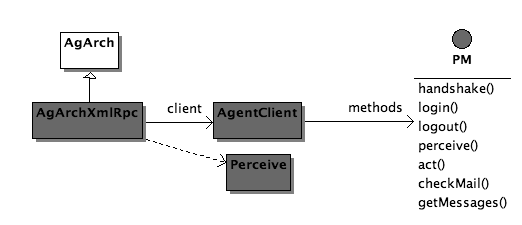
\includegraphics[width=100mm]{figuras/implXR-ag.png}
                \end{center}
                \caption{Diagrama da arquitetura do agente desenvolvido.}
                \label{fig-uml-ag}
\end{figure}

As mensagens de comunicação trocadas entre os agentes para uma comunicação
direta são tuplas com o seguinte formato: (i) identificador único da
mensagem; (ii) quem esta emitindo a mensagem, não é necessário preenche-lo;
(iii) tipo da mensagem sendo enviada, de preferência aos formatos
existentes do Jason; (iv) a quem se destina a mensagem sendo enviada; (v)
mensagem sendo enviada. Desta forma, quando se deseja dizer para um agente
(beltrano) que o disco esta gravado então a seguinte mensagem será enviada:
``<id42,,tell,beltrano,disco(gravado)>''. As crenças dos agentes,
entretanto, podem ser pensadas de duas formas: (i) o agente é responsável por
manter internamente suas crenças; (ii) o agente guarda suas crenças junto das
percepções utilizando as ações do ambiente.

Dadas essas duas opções, foi trabalhado com a segunda, que guarda as
percepções e crenças dos agentes no ambiente e parece ser um modelo mais
próximo do que existe hoje na plataforma Jason. Dessa forma, daqui por diante,
quando for mencionado, o dado de percepção este fará
alusão tanto a elementos percebidos do ambiente quanto crenças, conclusões ou
desejos feitos pelo agente. Assim, o ambiente é
responsável por armazenar as percepções dos agentes e por conhecer como as
ações dos agentes devem ser desempenhadas. Tanto o ambiente quanto o agente
possuem uma estrutura de classes semelhantes. Essa semelhança tem como
vantagem o ganho de velocidade quando, por ventura, for necessária alguma
modificação no futuro.

Dessa forma, o desenvolvimento do lado do ambiente seguiu um modelo parecido
com o do agente, conforme pode ser visto na Figura~\ref{fig-uml-env}. Essa
figura explica que o ambiente desenvolvido (classe \emph{EnvXmlRpc})
especializa o ambiente da plataforma (classe \emph{Environment}) para se
responsabilizar por quando ir no servidor. A classe \emph{Perceive} tem a
responsabilidade de traduzir as tuplas recebidas de e para o formato da
plataforma, conforme já explicado. A responsabilidade da classe
\emph{EnvironmentClient} é de ser o único meio de acessar o servidor externo.

Além disso, as interfaces servem para padronizar o acesso externo realizado.
Essa escolha pelas interfaces foi feita por dois motivos. O primeiro
foi deixar isolado os métodos que o servidor precisa responder.
Enquanto, o segundo foi tirar vantagem da técnica de reflexibilidade
que permite a construção de métodos que servem de \emph{proxy}. A
implementação do cliente feita na plataforma Jason pode ser visualizada no
Anexo~\ref{anexo-jason}.

\begin{figure}
               \begin{center}
               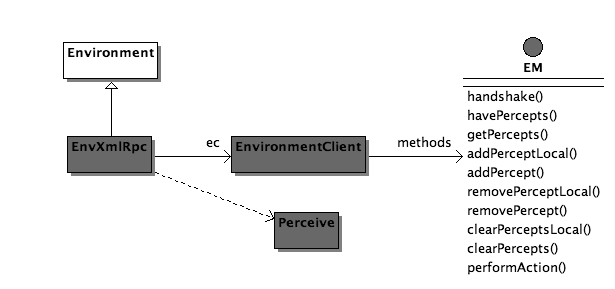
\includegraphics[width=100mm]{figuras/implXR-env.png}
                \end{center}
                \caption{Diagrama do ambiente desenvolvido.}
                \label{fig-uml-env}
\end{figure}

